%% This is file `elsarticle-template-1-num.tex',
%%
%% Copyright 2009 Elsevier Ltd
%%
%% This file is part of the 'Elsarticle Bundle'.
%% ---------------------------------------------
%%
%% It may be distributed under the conditions of the LaTeX Project Public
%% License, either version 1.2 of this license or (at your option) any
%% later version.  The latest version of this license is in
%%    http://www.latex-project.org/lppl.txt
%% and version 1.2 or later is part of all distributions of LaTeX
%% version 1999/12/01 or later.
%%
%% Template article for Elsevier's document class `elsarticle'
%% with numbered style bibliographic references
%%
%% $Id: elsarticle-template-1-num.tex 149 2009-10-08 05:01:15Z rishi $
%% $URL: http://lenova.river-valley.com/svn/elsbst/trunk/elsarticle-template-1-num.tex $
%%
\documentclass[preprint,12pt]{elsarticle}
\usepackage[utf8]{inputenc} % указывает кодировку документа
\usepackage[T2A]{fontenc} % указывает внутреннюю кодировку TeX 
\usepackage[main=russian,english]{babel} % указывает язык документа
%% Use the option review to obtain double line spacing
%% \documentclass[preprint,review,12pt]{elsarticle}

%% Use the options 1p,twocolumn; 3p; 3p,twocolumn; 5p; or 5p,twocolumn
%% for a journal layout:
%% \documentclass[final,1p,times]{elsarticle}
%% \documentclass[final,1p,times,twocolumn]{elsarticle}
%% \documentclass[final,3p,times]{elsarticle}
%% \documentclass[final,3p,times,twocolumn]{elsarticle}
%% \documentclass[final,5p,times]{elsarticle}
%% \documentclass[final,5p,times,twocolumn]{elsarticle}

%% The graphicx package provides the includegraphics command.
\usepackage{graphicx}
%% The amssymb package provides various useful mathematical symbols
\usepackage{amssymb}
\usepackage{amsmath}
%% The amsthm package provides extended theorem environments
%% \usepackage{amsthm}

%% The lineno packages adds line numbers. Start line numbering with
%% \begin{linenumbers}, end it with \end{linenumbers}. Or switch it on
%% for the whole article with \linenumbers after \end{frontmatter}.
\usepackage{lineno}

%% natbib.sty is loaded by default. However, natbib options can be
%% provided with \biboptions{...} command. Following options are
%% valid:

%%   round  -  round parentheses are used (default)
%%   square -  square brackets are used   [option]
%%   curly  -  curly braces are used      {option}
%%   angle  -  angle brackets are used    <option>
%%   semicolon  -  multiple citations separated by semi-colon
%%   colon  - same as semicolon, an earlier confusion
%%   comma  -  separated by comma
%%   numbers-  selects numerical citations
%%   super  -  numerical citations as superscripts
%%   sort   -  sorts multiple citations according to order in ref. list
%%   sort&compress   -  like sort, but also compresses numerical citations
%%   compress - compresses without sorting
%%
%% \biboptions{comma,round}

% \biboptions{}

%% Refs
\usepackage{hyperref}
\hypersetup{
     colorlinks   = true,
     citecolor    = blue
}
\usepackage[ruled,vlined]{algorithm2e}
\usepackage{booktabs}

% Переобозначение методов Эльзивера

\makeatletter

\def\ps@pprintTitle{%
   \let\@oddhead\@empty
   \let\@evenhead\@empty
   \let\@oddfoot\@empty
   \let\@evenfoot\@oddfoot
}

\usepackage{multicol}
\usepackage{lipsum}
\usepackage{mwe}

\renewenvironment{abstract}{\global\setbox\absbox=\vbox\bgroup
  \hsize=\textwidth\def\baselinestretch{1}%
  \noindent\unskip\textbf{Введение}
 \par\medskip\noindent\unskip\ignorespaces}
 {\egroup}

\def\keyword{%
  \def\sep{\unskip, }%
 \def\MSC{\@ifnextchar[{\@MSC}{\@MSC[2000]}}
  \def\@MSC[##1]{\par\leavevmode\hbox {\it ##1~MSC:\space}}%
  \def\PACS{\par\leavevmode\hbox {\it PACS:\space}}%
  \def\JEL{\par\leavevmode\hbox {\it JEL:\space}}%
  \global\setbox\keybox=\vbox\bgroup\hsize=\textwidth
  \normalsize\normalfont\def\baselinestretch{1}
  \parskip\z@
  \noindent\textit{Ключевые слова: квазиньютоновские методы \sep машинное обучение \sep глубинное обучение \sep глубокие нейронные сети }  % <--- Edit as necessary
  \raggedright                         % Keywords are not justified.
  \ignorespaces}
%

\begin{document}

\begin{frontmatter}

%% Title, authors and addresses

\title{Стохастические квазиньютоновские методы оптимизации в контексте глубоких нейронных сетей.}

%% use the tnoteref command within \title for footnotes;
%% use the tnotetext command for the associated footnote;
%% use the fnref command within \author or \address for footnotes;
%% use the fntext command for the associated footnote;
%% use the corref command within \author for corresponding author footnotes;
%% use the cortext command for the associated footnote;
%% use the ead command for the email address,
%% and the form \ead[url] for the home page:
%%
%% \title{Title\tnoteref{label1}}
%% \tnotetext[label1]{}
%% \author{Name\corref{cor1}\fnref{label2}}
%% \ead{email address}
%% \ead[url]{home page}
%% \fntext[label2]{}
%% \cortext[cor1]{}
%% \address{Address\fnref{label3}}
%% \fntext[label3]{}


%% use optional labels to link authors explicitly to addresses:
%% \author[label1,label2]{<author name>}
%% \address[label1]{<address>}
%% \address[label2]{<address>}

\author[mipt]{А. Жогов}
\ead{zhogov.aa@phystech.edu}
\author[mipt]{М. Сысак}
\ead{sysak.ma@phystech.edu}
\author[mipt]{Б. Усеинов}
\ead{useinov.br@phystech.edu}

\address[mipt]{Московский физико-технический институт (национальный исследовательский университет), Москва, Россия}

\begin{abstract}
%% Text of abstract

\end{abstract}

\begin{keyword}
%% keywords here, in the form: keyword \sep keyword

%% MSC codes here, in the form: \MSC code \sep code
%% or \MSC[2008] code \sep code (2000 is the default)

\end{keyword}

\end{frontmatter}

%%
%% Start line numbering here if you want
%%
% \linenumbers

%% main text
\section{Постановка задачи}
\label{S:1}
В машинном обучении по набору данных $\mathcal{X} = \{(\mathbf{x}_i, y_i)\}_{i=1}^n$, $\mathbf{x}_i~\in~\mathbb{R}^d$~--- вектор признаков $i$-го объекта, а $y_i \in \mathbb{Y}$~--- его метка, строится такое отображение $f\colon \, \mathbb{R}^n \rightarrow \mathbb{Y}$, чтобы наиболее точно выполнялось $\forall\, i \; f(x_i) \approx y_i$. 
В зависимости от конкретной задачи, $\mathbb{Y}$ может обозначать различные множества: так, в задаче регрессии чаще всего считается $\mathbb{Y} = \mathbb{R}$, в задаче классификации~--- $\mathbb{Y} = \{1, \dots, c\}$, где $c$~--- количество классов. 
Классический подход состоит в введении параметрического семейства функций $f\colon \, \mathbb{R}^n \times \mathbb{R}^m \rightarrow \mathbb{Y}'$, где $\mathbb{Y}'$~--- пространство предсказаний, часто не совпадающее с пространством меток, а $m$~--- размерность вектора параметров. 
Для подбора вектора $\theta \in \mathbb{R}^m$ вводится функция потерь $\mathcal{L}\colon \, \mathbb{Y}' \times \mathbb{Y} \rightarrow \mathbb{R}$. 
Оптимальное значение параметра задается как решение оптимизационной задачи
\begin{equation} \label{eq-opt-weight}
    \min_\theta F_\mathcal{X}(\theta) \triangleq \frac1n \sum_{i=1}^n \mathcal{L}(f(x_i, \theta), y_i).
\end{equation}

В данной статье будет рассмотрено глубинное обучение~--- раздел машинного обучения, относящийся к глубоким нейронным сетям.
Эта область накладывает серьезные ограничения на применимые для решения задачи~\eqref{eq-opt-weight} методы. 
В большинстве решаемых в этой области  задач целевая функция является дифференцируемой почти всюду, но не является выпуклой. 
Кроме того, часто размер выборки $n$ достаточно велик, что делает вычисление градиента $\nabla F_\mathcal{X}$ на каждой итерации численного метода неосуществимым. 
Вследствие этого стандартные алгоритмы первого порядка становятся неприменимыми. 
Для решения этой проблемы часто применяют подход минибатчей.
На каждой итерации случайно формируется подмножество исходной выборки $\mathcal{X}' = \{(x_{i_j}, y_{i_j})\}_{j=1}^s \subset \mathcal{X}, \, s \ll n$, и градиент считается по вспомогательной функции 
\begin{equation}
    F_{\mathcal{X}'}(\theta) \triangleq \frac1s \sum_{j=1}^s \mathcal{L}(f(x_{i_j}, \theta), y_{i_j}).
\end{equation} 
Как легко видеть, среднее значение функций $F_{\mathcal{X}'}$ по всем минибатчам совпадает с исходной функцией $F_\mathcal{X}$. 
Таким образом, вспомогательная функция является случайной величиной, матожидание которой равно исходной целевой функции. 
По этой причине часто к названиям методов, производящих вычисления над $F_{\mathcal{X}'}$ вместо $F_\mathcal{X}$, добавляют слово <<стохастический>>, поэтому здесь эти два термина используются взаимозаменяемо. 
Еще одно ограничение вытекает из большой размерности пространства параметров $\mathbb{R}^m$, что делает невозможным применение алгоритмов второго порядка, оперирующих полным гессианом целевой функции размерности $m \times m$. 
Эта проблема частично может быть решена применением квазиньютоновских методов, приближающих обратный гессиан с помощью вычисления градиента целевой функции, и позволяющих сократить расходы по памяти и время работы по сравнению с методами второго порядка.

В этой статье будет рассмотрено три варианта применения стохастических модификаций квазиньютоновских методов в глубинном обучении, для сравнения будут использованы два стандартных для области подхода, наиболее часто используемых при решении большинства задач, свазанных с нейронными сетями:
\begin{enumerate}
    \item Стохастический градиентный спуск (SGD)~--- классический метод оптимизации, используемый в решении задач машинного обучения, модификация стандартного градиентного спуска.
    \item Adam~\cite{adam}~--- распространенный метод оптимизации в контексте нейронных сетей, часто используется как базовое решение при выборе алгоритма для конкретной задачи. 
    \item SGD-BB~\cite{BB-DL}--- стохастическая модификация метода Barzilai-Borwein, представляющая из себя вариант выбора шага в SGD.
    \item Multi-Batch BFGS~\cite{multibatchLBFGS}~--- стохастическая модификация наиболее известного квазиньютоновского метода BFGS.
    \item Sampled BFGS~\cite{sampledbfgs}~--- модификация того же метода, в которой используется другой подход к  построению приближения обратного гессиана.
\end{enumerate}
\section{Методы}
\label{S:2}
Рассматриваемые ниже методы будут сравниваться двумя способами: на фиксированной задаче будет рассматриваться значение некоторой метрики качества (подробнее в разделе~\ref{S:3}), достигнутой за фиксированное число эпох, а также будет измеряться время, затрачиваемое на фиксированное число эпох обучения. 
Эпохой называют группу из числа итераций, равного отношению размера всей выборки $|\mathcal{X}|$ к размеру минибатча $|\mathcal{X}'|$.
\subsection{SGD}
SGD, или стохастический градиентный спуск, представляет из себя простейший метод оптимизации, используемый в машинном обучении. 
На каждой итерации генерируется минибатч $\mathcal{X}'$, после чего параметры обновляются по формуле
\begin{equation*}
    \theta_{k+1} = \theta_k - \eta_k \nabla F_{\mathcal{X}'} (\theta_k)
\end{equation*}
Здесь последовательность длин шага $\{\eta_k\}$~--- параметр алгоритма, к выбору которого есть несколько распространенных подходов:
\begin{itemize}
    \item $\eta_k \equiv \eta$~--- фиксированный шаг. Стандартный выбор $\eta = 0.001$. В разделе~\ref{S:3} рассматривается этот подход.
    \item Убывающая последовательность $\eta_{k+1} < \eta_k$. На практике, в задачах глубинного обучения влечет более быструю сходимость по итерациям.
    \item <<Понижение шага на плато>>~--- стратегия выбора шага, специфичная для глубинного обучения. Примером является умножение шага на фиксированную константу $\alpha \in (0, 1)$ после фиксированного числа $r$ эпох без достаточного уменьшения значения целевой функции или метрики качества.
\end{itemize}
Каждая итерация алгоритма требует $O(m)$ времени, $O(m)$ памяти и $1$ вычисления градиента.
\subsection{Adam}
\begin{algorithm}[H]\label{Adam}
\caption {Adam\newlineЗдесь все операции с векторами покомпонентные;\newline$\beta_i^{t+1}$ обозначает возведение числа $\beta_i$ в степень $t + 1$, $i \in \{1, 2\}$.}
\SetKwInOut{Input}{Input}
\SetKwInOut{Output}{Output}
\SetAlgoLined
\Input{Число итераций $N$ \newline
        Размер шага $\eta$ \newline
        Экспоненциальные скорости затухания $\beta_1, \beta_2 \in [0, 1)$ \newline
        Начальное приближение $\theta_0$ \newline
        Поправка на численную неустойчивость $\varepsilon$}
\Output{Итоговое значение параметра $\theta_N$}
 $m_0 \leftarrow 0$\\
 $v_0 \leftarrow 0$\\
 \For{$t = 0, 1, \dotsc, N-1$}{
  Сгенерировать минибатч $\mathcal{X}_t' \subset \mathcal{X}$\\
  $g_{t+1} \leftarrow \nabla F_{\mathcal{X}_t'}(\theta_t)$\\
  $m_{t+1} \leftarrow \beta_1 \cdot m_t + (1 - \beta_1)\cdot g_{t+1}$ \\
  $v_{t+1} \leftarrow \beta_2 \cdot v_t + (1 - \beta_2)\cdot g_{t+1}^2$\\
  $m_{t+1} \leftarrow m_{t+1} / (1 - \beta_1^{t+1})$\\
  $v_{t+1} \leftarrow v_{t+1} / (1 - \beta_2^{t+1})$\\
  $\theta_{t+1} \leftarrow \theta_t - \eta \cdot m_{t+1}/(\sqrt{v_{t+1}} + \varepsilon)$
 }
 \Return{$\theta_N$}
\end{algorithm}
В алгоритме~\ref{Adam} описан псевдокод метода Adam, представленного в \cite{adam}. 
В этом методе на каждой итерации обновляются скользящие экспоненциальные средние, то есть величины вида
\[
    \overline{x}_{k+1} = \gamma\overline{x}_k + (1 - \gamma)x_{k+1}
\]
для коэффициента $\gamma \in (0, 1)$. 
Такие значения поддерживаются алгоритмом для градиента с коэффициентом $\beta_1$ и для покомпонентного квадрата градиента с коэффициентом $\beta_2$. 
Стандартным выбором является $\beta_1 = 0.9$ и $\beta_2 = 0.999$. 
В оригинальной статье было показано, что полученные величины являются оценками градиента и его квадрата по всей выборке, смещенными на коэффициенты $(1 - \beta_1^{t+1})$ и $(1 - \beta_2^{t+1})$ соответственно. 
Поэтому для получения несмещенных оценок следующим шагом обе величины делятся на соответствующие им коэффициенты. 
Наконец, вектор параметров обновляется на величину $-\eta \cdot m_{t+1} / (\sqrt{v_{t+1}} + \varepsilon)$. 
Поправка $\varepsilon$ здесь нужна для численной стабильности на случай близких к нулю градиентов. 
Стандартным выбором является $\varepsilon = 10^{-8}$. 
Для длины шага стандартный выбор $\eta = 0.001$. 
От SGD такое правило отличается тем, что вместо градиента теперь используется скользящее среднее градиентов по всем итерациям, покомпонентно деленное на корень из скользящего среднего их квадратов. 
Основная мотивация состоит в том, что подобное масштабирование позволяет увеличить шаг вдоль направлений с маленьким градиентом, предотвращая сходимость к седловым точкам.

Данный метод имеет те же асимптотики по времени и памяти и требует такого же количества вычислений градиента, что и SGD.
\subsection{SGD-BB}
\begin{algorithm}[H]\label{SGD-BB}
\caption {SGD-BB}
\SetKwInOut{Input}{Input}
\SetKwInOut{Output}{Output}
\SetAlgoLined
\Input{Число эпох $K$ \newline
        Число шагов в эпохе $T$ \newline
        Размер шага $\eta_0 = \eta_1$ \newline
        Экспоненциальная скорость затухания $\beta \in (0, 1]$ \newline
        Начальное приближение $\theta_{0, 0}$ \newline
        Корректирующие $\hat{\eta}_k$ параметры $\tau_0$, $\tau_{\text{min}}$, $\tau_{\text{max}}$
        }
\Output{
        Итоговое значение $\theta_{K, 0}$
    }
 \For{$k = 0, \ldots, K-1$}{
  \If{$k > 1$}{
    $y_{k-1} \leftarrow g_{k-1, T} - g_{k-2, T}$\\
    $s_{k-1} \leftarrow \frac{1}{T}(\theta_{k-1, T} - \theta_{k-2, T})$ \\
    $\eta_{k} \leftarrow \frac{\|s_{k-1}\|^2}{|s_{k-1}^Ty_{k-1}|}$ \\
    $\hat{\eta}_k = 
    \begin{cases}
        \eta_k & \text{если } \eta_k \in \left[\frac{\tau_{\text{min}}}{k+1}, \frac {\tau_{\text{max}}}{k+1}\right], \\
        \frac{\tau_0}{k+1} & \text{иначе.}
    \end{cases}$\\
  }
  $g_{k, 0} \leftarrow 0$ \\
 \For{$t = 0, \ldots, T-1$} {
    Сгенерировать минибатч $\mathcal{X}_{k, t}' \subset \mathcal{X}$\\ 
    $\theta_{k, t+1} \leftarrow \theta_{k, t} - \hat{\eta}_k \nabla F_{\mathcal{X}_{k, t}'}(\theta_{k, t})$ \\
    $g_{k, t+1} = (1 - \beta) g_{k, t} + \beta \nabla F_{\mathcal{X}_{k, t}'}(\theta_{k, t})$ \\
 }
 $\theta_{k+1, 0} \leftarrow \theta_{k, T}$ \\
 }
 \Return{$\theta_{K, 0}$}
\end{algorithm}
Главной идеей алгоритма стандартного алгоритма BB является расчет размера шага с использованием информации с предыдущих итераций. 
В данном методе гессиан целевой функции аппроксимируется матрицей $B_t = \eta_t^{-1}I$, где $\eta_t^{-1}$ определяется как значение, при котором $B_t$ наиболее хорошо удовлетворяет квазиньютоновскому уравнению
\[
    B_ts_t = y_t,
\]
где $s_t = \theta_{t+1} - \theta_t$ и $y_t = \nabla F_\mathcal{X}(\theta_{t+1}) - \nabla F_\mathcal{X}(\theta_t)$.
Конкретно, $\eta_t$ выбирается равным решению следующей задачи оптимизации:
\begin{align*}
    \min_{\eta_{t}}\| \eta_t^{-1}s_{t}-y_{t}\|_2^2
\end{align*}
В явной форме оно записывается в виде
$$\eta_{t} = \frac{\|s_{t}\|_2^2}{s_{t}^Ty_{t}}$$
Модификация SGD-BB, представленная в~\cite{BB-DL} и алгоритм которой показан в процедуре~\ref{SGD-BB}, использует идею выделения минибатчей и рассчитывает значение размера шага ${\eta}_{k+1}$ следующей эпохи при помощи $T$ итераций, на которых используется размер шага текущей эпохи~--- ${\eta}_{k}$. 
Обновление $\theta_{k, t}$ (k~--- индекс эпохи, t~--- индекс времени внутри эпохи) происходит по правилу
$$\theta_{k, 0} = \theta_{k-1, T},~\theta_{k, t+1} = \theta_{k, t} - {\eta}_k \nabla F_{\mathcal{X}_{k, t}'}(\theta_{k, t})$$
Градиент $g_{k, t}$, использующийся для нахождения ${\eta_k}$, оценивается как и в методе Adam~\ref{Adam} при помощи экспоненциального скользящего среднего
$$g_{k, t+1} = (1 - \beta) g_{k, t} + \beta \nabla F_{\mathcal{X}_{k, t}'}(\theta_{k, t})$$
Тогда разность градиентов между эпохами считается как
$$y_k = g_{k, T} - g_{k-1, T}$$
А разность точек между двумя эпохами определяется как
$$s_k = T^{-1}(\theta_{k, T} - \theta_{k-1, T})$$
Определенные так $s_k, y_k$ дают размер шага следующей эпохи
$$\eta_{k+1} = \frac{\|s_k\|_2^2}{|s_k^Ty_k|}$$
Для обеспечения сходимости метода значения $\eta_k$ корректируются при помощи заданных параметров $\tau_0, \tau_{\text{min}}, \tau_{\text{max}}$
$$\hat{\eta}_k = \begin{cases}
        \eta_k & \text{если } \eta_k \in \left[\frac{\tau_{\text{min}}}{k+1}, \frac {\tau_{\text{max}}}{k+1}\right], \\
        \frac{\tau_0}{k+1} & \text{иначе.}
    \end{cases}$$

Стандартным выбором размера шага является $\eta_0 = \eta_1 = 0.001$. 
Число шагов в эпохе $T$ целесообразно принять равным отношению размера выборки к размеру одного минибатча $|\mathcal{X}|/|\mathcal{X}'|$. 
В качестве коэффициента $\beta$ авторы оригинальной статьи предлагают отношение $4 / T$. 
Для корректирующих параметров целесообразный вариант представляет из себя набор $\tau_0 = 0.001$, $\tau_\text{min} = 10^{-5}$, $\tau_\text{max} = 1$.

Каждая итерация внутреннего цикла алгоритма требует $O(m)$ памяти и времени и $1$ вычисления градиента. 
Вне этого цикла на каждой эпохе происходят вычисления с теми же затратами по памяти и времени, но без вычислений градиента.

\subsection{Multi-Batch LBFGS}
\begin{algorithm}[H]\label{twolooprec}
\caption {two\_loop\_recursion}
\SetKwInOut{Input}{Input}
\SetKwInOut{Output}{Output}
\SetAlgoLined
\Input{Вектор $\mathbf{x}$\newline
       Набор пар $\{(y_i, s_i)\}_{i=k-p}^{k-1}$
        }
\Output{Произведение $H_k\mathbf{x}$}
 \For{$i = k-1, k-2, \dotsc, k-p$}{
  $\alpha_i \leftarrow s_i^\top \mathbf{x} / s_i^\top y_i$\\
  $\mathbf{x} \leftarrow \mathbf{x} - \alpha_i y_i$\\
 }
 $\mathbf{r} \leftarrow \dfrac{s_{k-1}^\top y_{k-1}}{y_{k-1}^\top y_{k-1}}\mathbf{x}$\\
 \For{$i = k-p, k-p+1, \dotsc, k-1$} {
    $\beta \leftarrow \dfrac{y_i^\top \mathbf{r}}{s_i^\top y_i}$\\
    $\mathbf{r} \leftarrow \mathbf{r} + s_i(\alpha_i - \beta)$\\
 }
 \Return{$\mathbf{r}$}
\end{algorithm}
Основная идея алгоритма Multi-Batch LBFGS, предложенного в \cite{multibatchLBFGS}, состоит в построении на каждой итерации оценки обратного гессиана $H_k$ и обновлении вектора параметров по правилу
\[ 
    \theta_{k+1} = \theta_k - \eta H_k \nabla F_{\mathcal{X}_k'}(\theta_k),
\]
где $\mathcal{X}_k'$~--- минибатч. 
В отличие от BB, здесь приближение обратного гессиана $H_k$ строится таким образом, чтобы оно строго удовлетворяло квазиньютоновскому уравнению
\[s_{k+1} = H_{k+1}y_{k+1},\]
где
\[y_{k+1} = \nabla F_{\mathcal{X}_{k+1}' \cap \mathcal{X}_k'}(\theta_{k+1}) - \nabla F_{\mathcal{X}_{k+1}' \cap \mathcal{X}_k'}(\theta_k) \quad s_{k+1} = \theta_{k+1} - \theta_k\]
В дальнейшем будем обозначать $O_k = \mathcal{X}_{k+1}' \cap \mathcal{X}_k'$. 
Такие условия накладывают ограничение на процедуру генерации батчей: требуется, чтобы два батча на соседних итерациях имели пересечение фиксированного размера $|O_k| = l < s = |\mathcal{X}_k'|$. 
Это требование обусловлено тем, что на практике при вычислении градиентов для $y_{k+1}$ по разным подмножествам выборки $\mathcal{X}$ оценка обратного гессиана $H_k$ становится неустойчивой. 
Метод хранит последние $p$ пар $(y_i, s_i)$, и по ним вычисляет произведение $H_k \nabla F_{\mathcal{X}_k'}(\theta_k)$ с помощью процедуры two\_loop\_recursion~\cite{numopt}, псевдокод которой вынесен в алгоритм~\ref{twolooprec}. 
В конце каждой итерации пара $(y_{k - p}, s_{k - p})$ заменяется на новую пару $(y_k, s_k)$. 
Псевдокод всего метода находится в алгоритме~\ref{MB-LBFGS}.\\
\begin{algorithm}[H]\label{MB-LBFGS}
\caption {Multi-Batch LBFGS}
\SetKwInOut{Input}{Input}
\SetKwInOut{Output}{Output}
\SetAlgoLined
\Input{Число итераций $N$ \newline
Начальное приближение $\theta_0$ \newline
Размер памяти $p$ \newline
Размер пересечения минибатчей $l$ \newline
Размер шага $\eta$}
\Output{Итоговое значение параметра $\theta_N$}
 Сгенерировать минибатч $\mathcal{X}_0'$\\
 $C \leftarrow \varnothing$\\
 \For{$k = 0, 1, \dotsc, N-1$}{
  $g_k \leftarrow \nabla F_{\mathcal{X}_k'}(\theta_k)$\\
  $p_k \leftarrow \text{two\_loop\_recursion}(g_k, C)$\\
  $\theta_{k+1} \leftarrow \theta_k - \eta \cdot p_k$\\
  Создать минибатч $\mathcal{X}_{k+1}'$\\
  $O_k \leftarrow \mathcal{X}_{k+1}' \cap \mathcal{X}_k'$\\
  $s_{k+1} \leftarrow \theta_{k+1} - \theta_k$\\
  $y_{k+1} \leftarrow \nabla F_{O_k}(\theta_{k+1}) - \nabla F_{O_k}(\theta_k)$\\
  \eIf{$k \ge p$}{
   $C \leftarrow C \cup \{(y_{k+1}, s_{k+1})\} \setminus \{(y_{k+1-p}, s_{k+1-p})\}$
  }{
   $C \leftarrow C \cup \{(y_{k+1}, s_{k+1})\}$
  }
 }
\end{algorithm}
Стандартным выбором $p$ являются числа из отрезка $[2, 20]$, отношение размера пересечения минибатчей к размеру одного минибатча $l/s$ может быть любым числом из интервала $(0, 0.5)$, стандартный выбор~--- $0.25$. 
Стандартный размер шага $\eta = 1$, что мотивировано наличием матрицы $H_k$, которая представляет из себя альтернативу умножению градиента на скаляр и сама по себе играет роль <<длины шага>>.

Каждая итерация алгоритма требует $O(mp)$ времени и памяти, а также $3$ вычислений градиента.
\subsection{Sampled LBFGS}
\begin{algorithm}[H]\label{sampleCurvature}
\caption {C\_generate}
\SetKwInOut{Input}{Input}
\SetKwInOut{Output}{Output}
\SetAlgoLined
\Input{Начальное приближение $\theta_0$ \newline
Минибатч $\mathcal{X}'$ \newline
Размер памяти $p$ \newline
Радиус отбора $\rho$}
\Output{Множество пар $C$\newline
        Градиент в начальной точке $\nabla F_{\mathcal{X}'}(\theta_0)$}
 $g \leftarrow \nabla F_{\mathcal{X}'}(\theta_0)$\\
 $C \leftarrow \varnothing$\\
 \For{$i = 1, 2, \dotsc, p$}{
  Сгенерировать случайный $\sigma \in \mathbb{R}^m$, $\|\sigma\|_2 = 1$\\
  $\theta \leftarrow \theta_0 + \rho\cdot\sigma$\\
  $s \leftarrow \theta_0 - \theta$\\
  $y \leftarrow  g - \nabla F_{\mathcal{X}'}(\theta)$\\
  $C \leftarrow C \cup \{(y, s)\}$
 }
 \Return{$C$, $g$}
\end{algorithm}
Данный метод, предложенный в \cite{sampledbfgs}, представляет из себя альтернативную модификацию метода LBFGS. 
Его отличие от Multi-Batch версии в том, что, вместо истории пар $(y_i, s_i)$ по последним $p$ итерациям, на каждой итерации генерируется набор из $p$ случайных пар $C = \{(y_i, s_i)\}_{i=1}^p$ с помощью процедуры~\ref{sampleCurvature}. 
Это позволяет снять ограничение на пересечение последовательных минибатчей, но при этом увеличивает количество операций за одну итерацию алгоритма. 
Пары $(y_i, s_i)$ задают информацию о кривизне графика целевой функции, поэтому их вычисление в малой окрестности текущей точки позволяет получить приемлемую с практической точки зрения локальную оценку обратного гессиана и избежать проблем с устойчивостью, которые были упомянуты в предыдущем разделе. 
Алгоритм вычисления приближения обратного гессиана $H_k$ совпадает с таковым для предыдущего метода и описан в процедуре~\ref{twolooprec}. Псевдокод метода Sampled LBFGS приведен в~\ref{sampledLBFGS}.

\begin{algorithm}[H]\label{sampledLBFGS}
\caption {Sampled LBFGS}
\SetKwInOut{Input}{Input}
\SetKwInOut{Output}{Output}
\SetAlgoLined
\Input{Число итераций $N$ \newline
Начальное приближение $\theta_0$ \newline
Размер памяти $p$ \newline
Радиус отбора $\rho$ \newline
Размер шага $\eta$}
\Output{Итоговое значение параметра $\theta_N$}
 \For{$k = 0, 1, \dotsc, N-1$}{
  Сгенерировать минибатч $\mathcal{X}_k'$\\
  $C, g_k \leftarrow \text{C\_generate}(\theta_k, \mathcal{X}_k', p, \rho)$\\
  $p_k \leftarrow \text{two\_loop\_recursion}(g_k, C)$\\
  $\theta_{k+1} \leftarrow \theta_k - \eta \cdot p_k$\\
 }
\end{algorithm}

Стандартные значения для $p$ и $\eta$ совпадают с соответствующими значениями для предыдущего метода. Для радиуса отбора простейшим вариантом является $\rho = 1$.

Асимптотики по времени и памяти данного метода совпадают с Multi-Batch LBFGS. 
При этом за итерацию градиент вычисляется $p+1$, что при больших $p$ является более плохим показателем, чем в случае с Multi-Batch модификацией, которая требует $3$ вычислений.
\section{Эксперименты}
\label{S:3}
В данном разделе рассматривается несколько примеров применения вышеописанных методов к задаче классификации. В каждом эксперименте для конкретной задачи строится и обучается нейронная сеть подходящей архитектуры. В качестве метрики качества обученной модели используется доля правильных ответов на отложенной выборке $\mathcal{X}_\text{test}$, данные из которой модель <<не видела>> во время обучения. Эту величину будем обозначать Acc (от слова accuracy). Такой подход к оцениванию качества моделей типичен для машинного обучения.
\subsection{MNIST}
В этом эксперименте метод SGD-BB сравнивается с SGD и Adam на примере оптимизации полносвязной нейронной сети на наборе данных MNIST \cite{MNIST}. Задача состоит в определении цифры, изображенной на картинке размера $28 \times 28$.
\begin{table}[h!]
\caption{MNIST}
\centering
\begin{tabular}{lrrrr}
\toprule
Метод &  Время, мин &  Acc, 5 эпох &  Acc, 10 эпох &  Acc, 15 эпох \\
\midrule
      SGD &  2.65 &  89.68 &   91.58 &   92.75 \\
     Adam &  3.00 &  96.59 &   97.04 &   97.02 \\
   SGD-BB &  2.75 &  91.23 &   96.52 &   97.67 \\
\bottomrule
\end{tabular}
\end{table}
\begin{figure*}[ht!]
    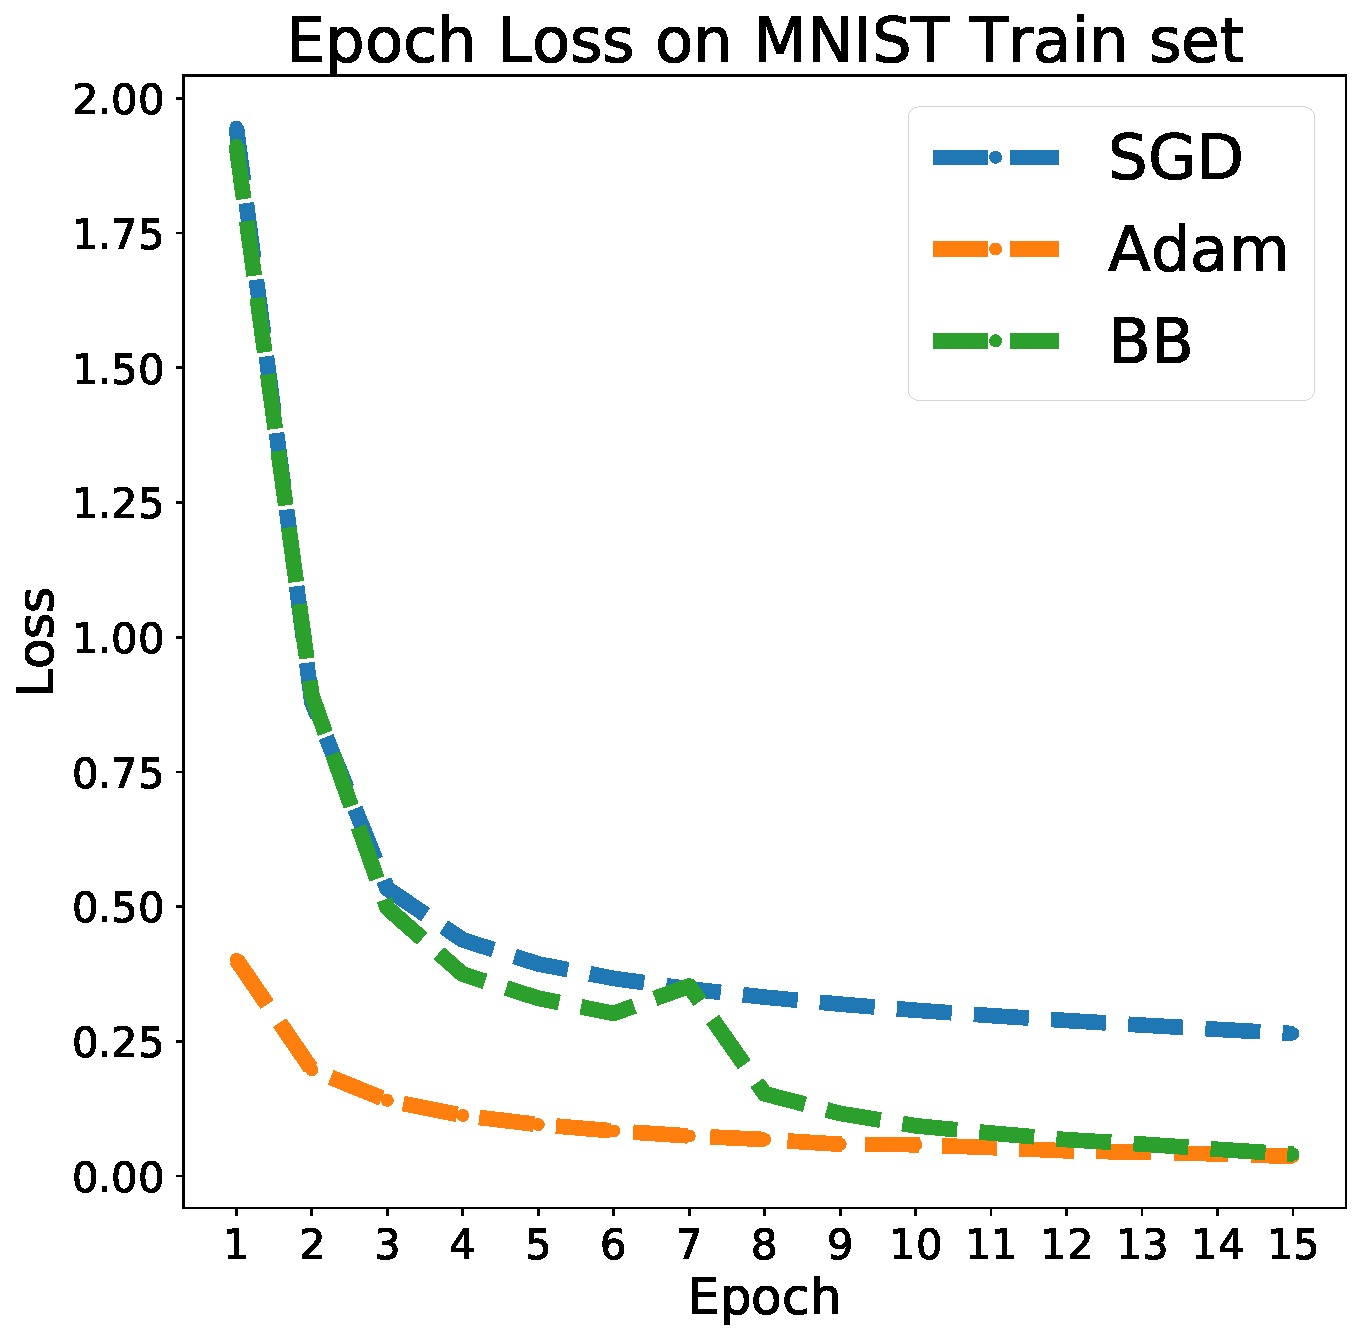
\includegraphics[height=.33\textwidth]{mnist_train_losses (3).pdf}\hfill
    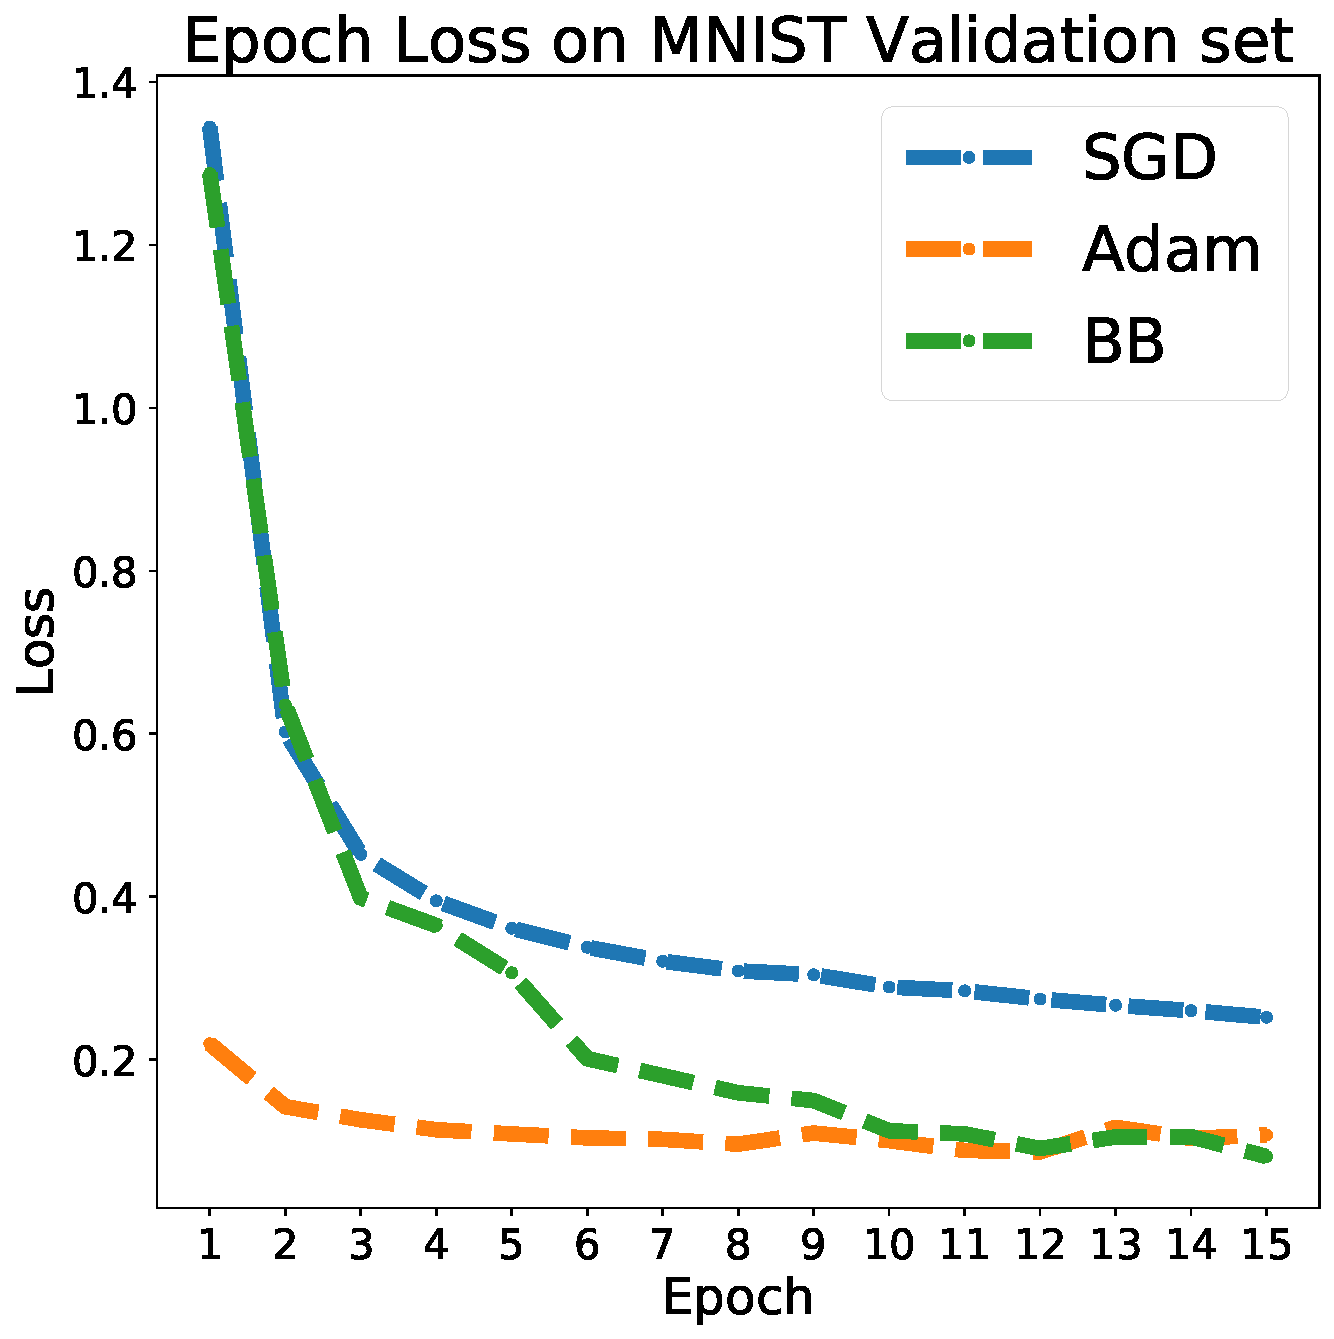
\includegraphics[height=.33\textwidth]{mnist_val_losses (3).pdf}\hfill
    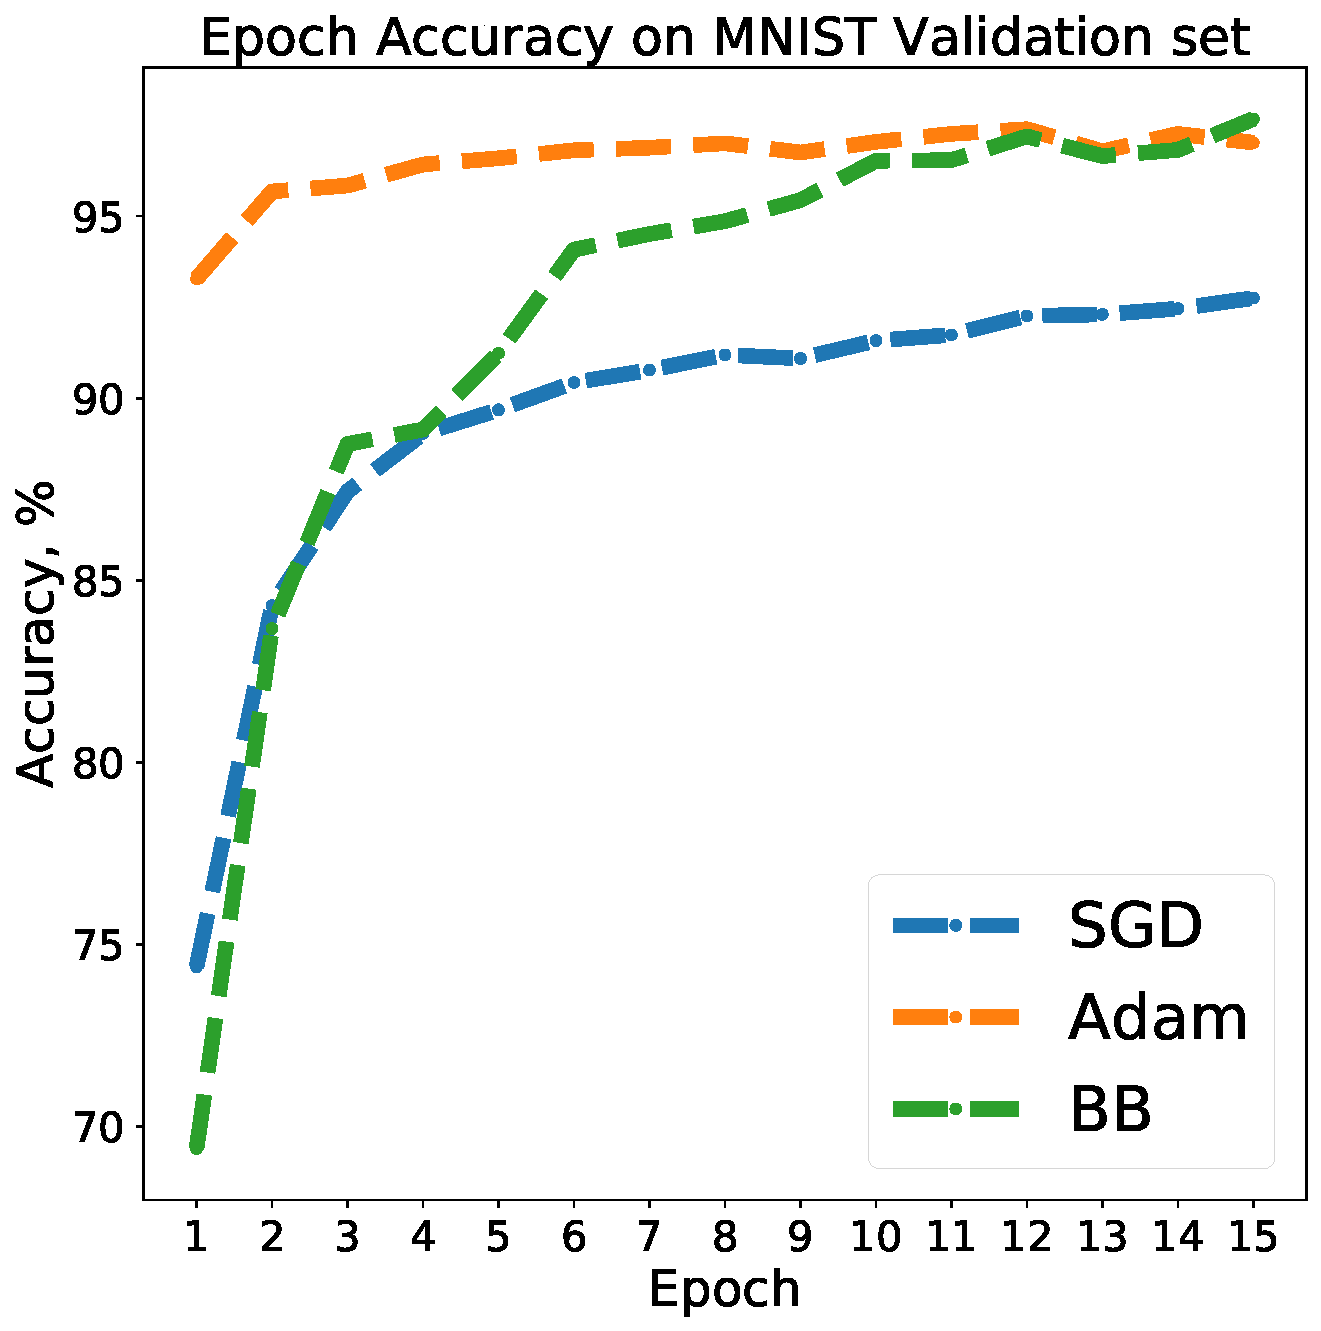
\includegraphics[height=.33\textwidth]{mnist_val_accuracy (3).pdf}
\end{figure*}

По времени все три алгоритма практически идентичны, но Adam работает немного дольше, поскольку он делает больше вычислений на каждой итерации. 
По достигаемой метрике качества Adam резко превосходит два других алгоритма на первых итерациях, но на последних эпохах BB достигает сравнимого качества с ним качества. 
При этом видно явное превосходство выбора шага по правилу BB (в методе SGD-BB) перед константным значением (в методе SGD).


\subsection{CIFAR-10}
В этом эксперименте MultiBatch LBFGS и SGD-BB сравниваются с Adam и SGD при оптимизации сверточной нейронной сети на датасете CIFAR-10 \cite{CIFAR10}. 
Набор данных состоит из фотографий размером $32 \times 32$, которые необходимо классифицировать на $10$ классов.
\begin{table}[h!]
\caption{CIFAR-10}
\centering
\begin{tabular}{lrrrr}
\toprule
Метод &  Время, мин &  Acc, 5 эпох &  Acc, 10 эпох &  Acc, 15 эпох \\
\midrule
    MB-LBFGS &  6.99 &  40.34 &   43.12 &   45.98 \\
     Adam &  5.48 &  52.83 &   58.79 &   60.72 \\
      SGD &  5.18 &  10.13 &   15.27 &   23.69 \\
       SGD-BB &  5.19 &  13.61 &   44.20 &   51.74 \\
\bottomrule
\end{tabular}
\end{table}
\begin{figure*}[ht!]
    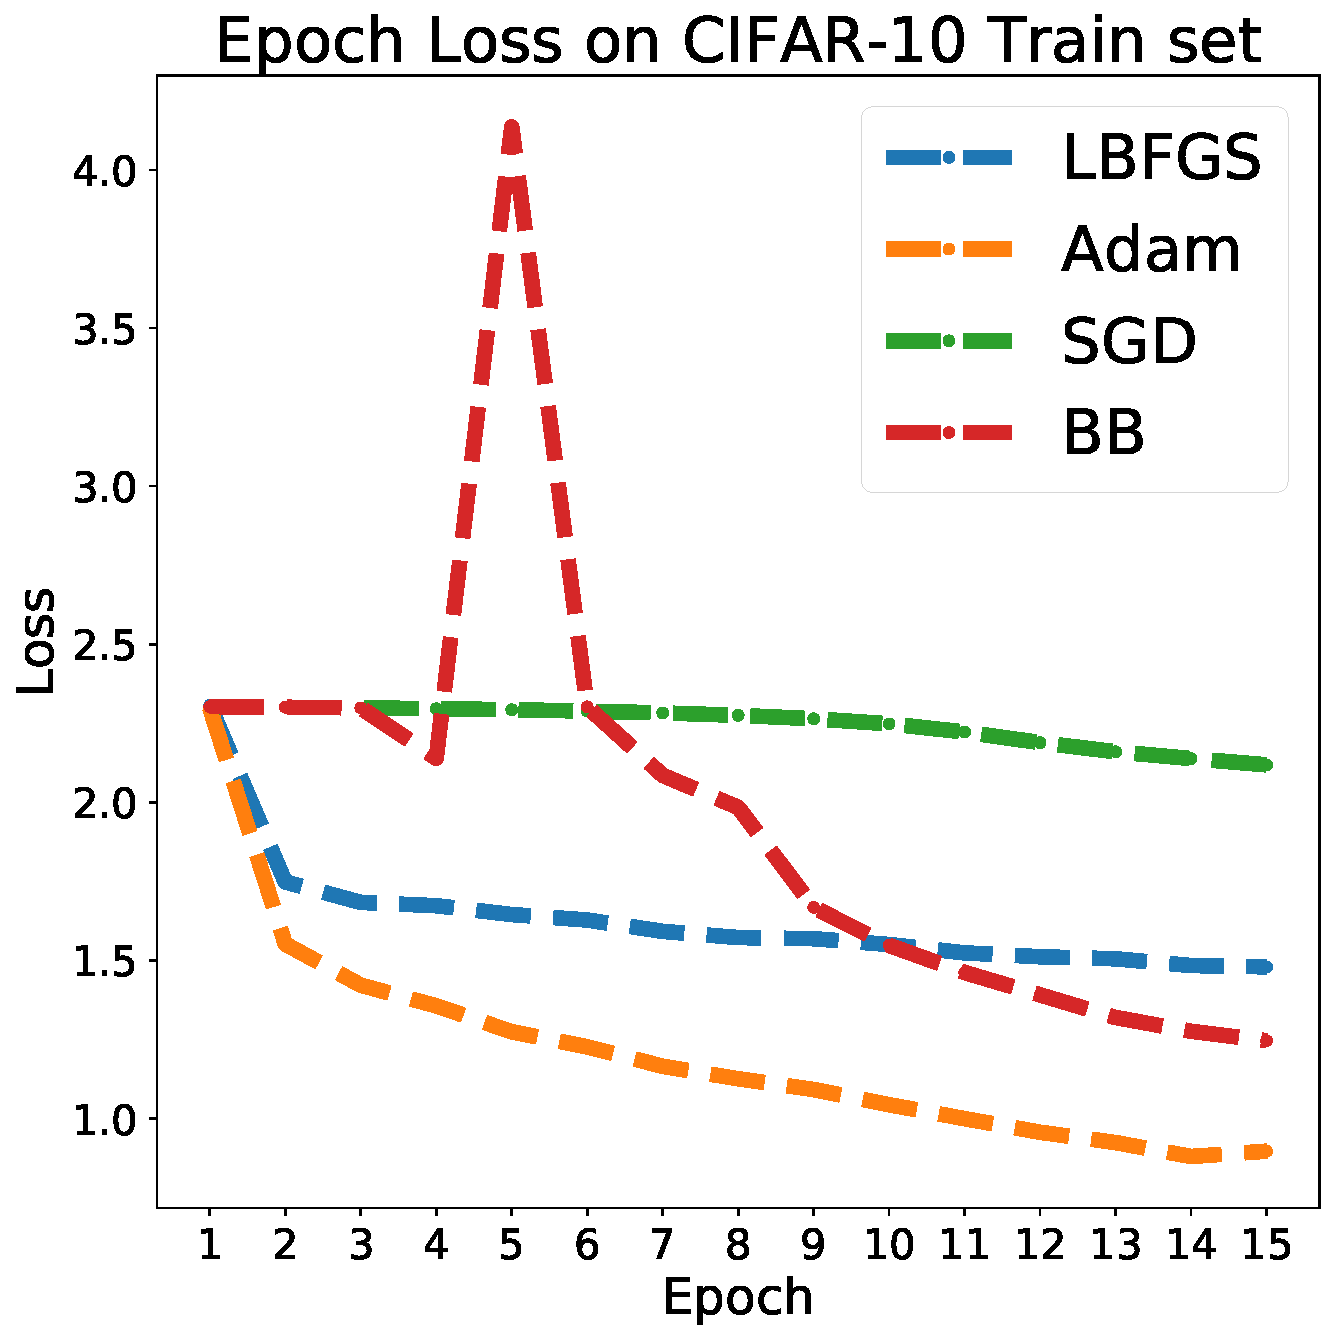
\includegraphics[height=.33\textwidth]{cifar_train_losses.pdf}\hfill
    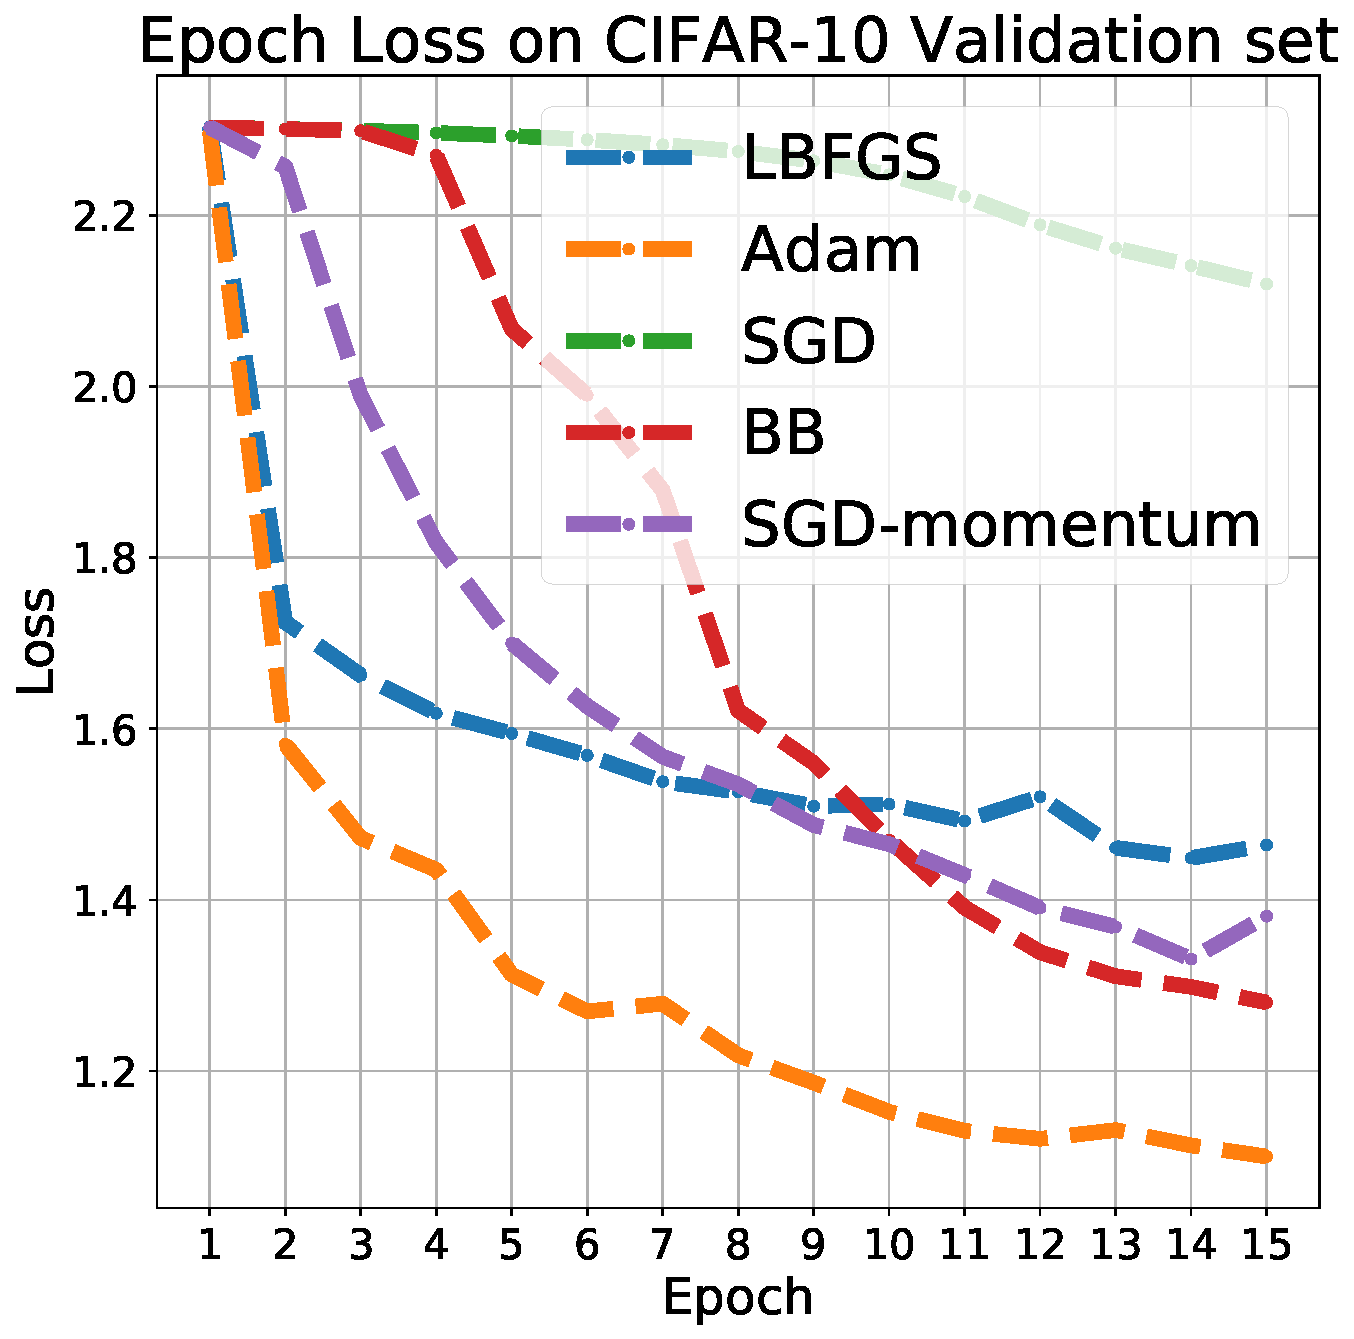
\includegraphics[height=.33\textwidth]{cifar_val_losses.pdf}\hfill
    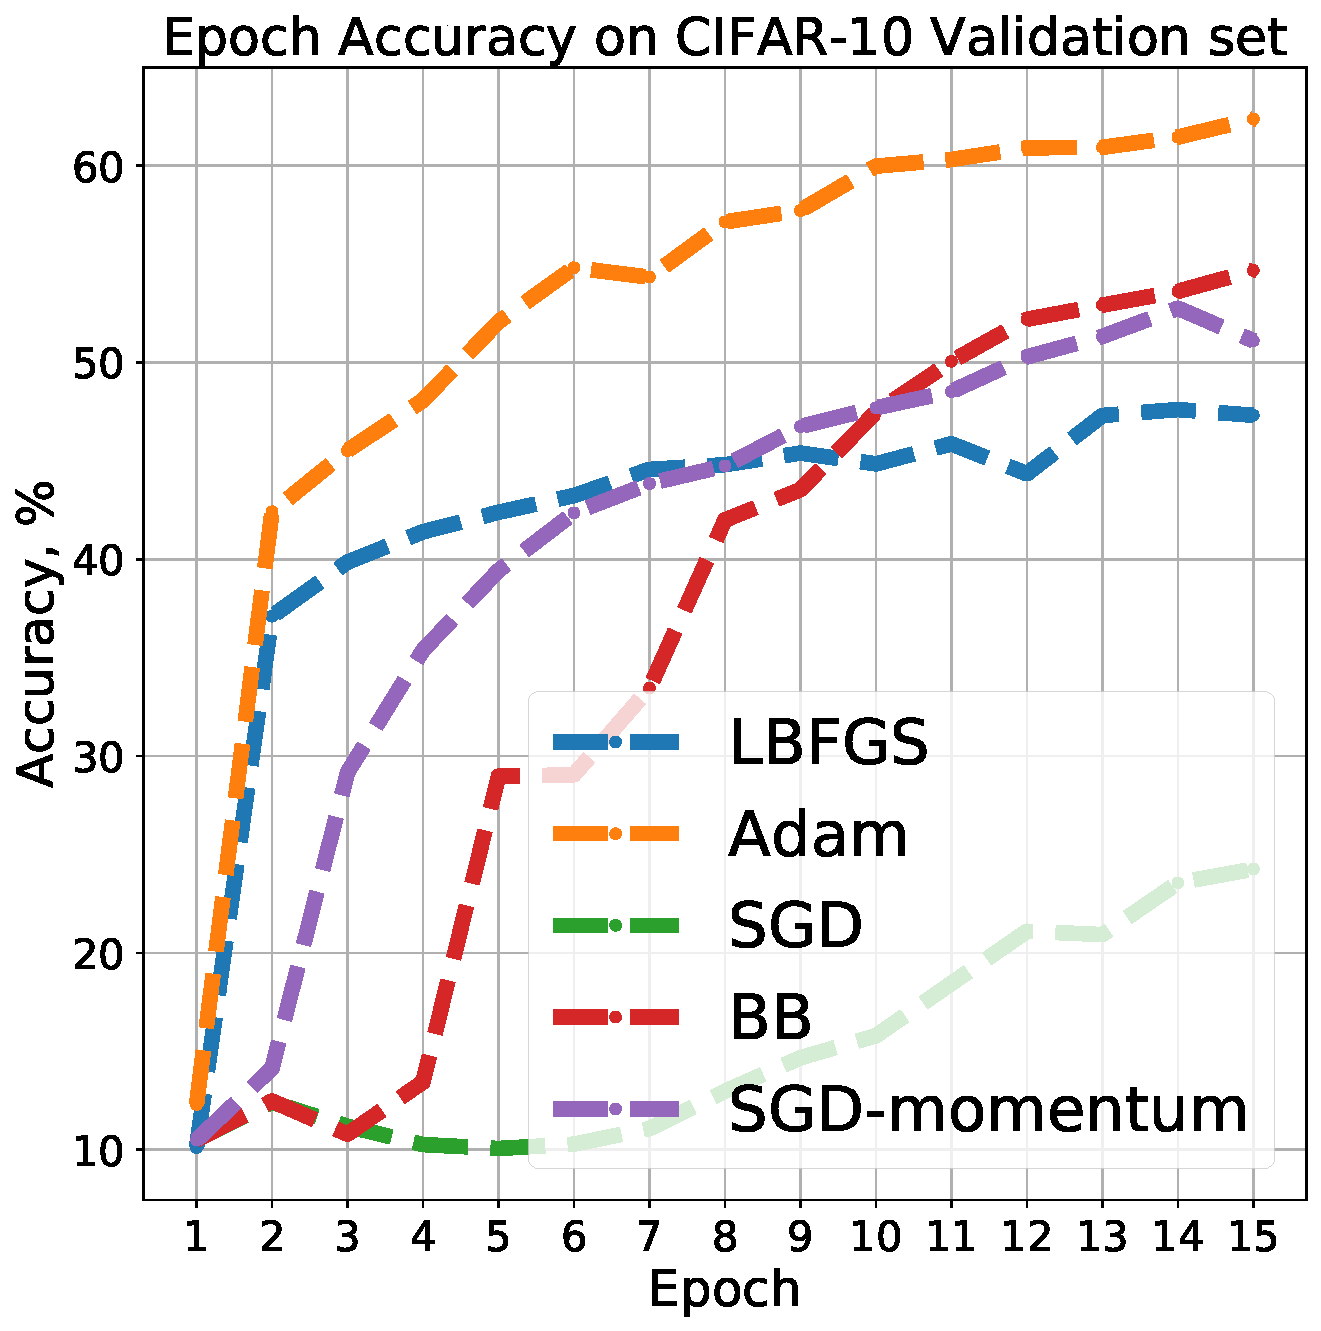
\includegraphics[height=.33\textwidth]{cifar_val_accuracy.pdf}
\end{figure*}

Как и в прошлом эксперименте, последние три алгоритма практически не отличаются по затрачиваемому времени, в то время как MB-LBFGS работает дольше на четверть. 
Это объясняется тем, что этот метод требует нескольких вычислений градиента на каждой итерации, а каждое вычисление требует двух проходов по нейросети. 
По достигаемой точности SGD показывает результат резко хуже остальных алгоритмов, что является распространенным явлением при использовании постоянного шага в глубоких нейронных сетях. 
Adam и BB показывают похожие результаты, но первый оказывается предпочтительнее.
MB-LBFGS дает более плохой результат, чем предыдущие два алгоритма, что может быть вызвано
плохим выбором гиперпараметров.
\section{Заключение}
\label{S:4}

%% The Appendices part is started with the command \appendix;
%% appendix sections are then done as normal sections
%% \appendix

%% \section{}
%% \label{}

%% References
%%
%% Following citation commands can be used in the body text:
%% Usage of \cite is as follows:
%%   \cite{key}          ==>>  [#]
%%   \cite[chap. 2]{key} ==>>  [#, chap. 2]
%%   \citet{key}         ==>>  Author [#]

%% References with bibTeX database:

% \bibliographystyle{model1-num-names}

%% New version of the num-names style
\bibliographystyle{elsarticle-num-names}
\bibliography{bibliography.bib}

%% Authors are advised to submit their bibtex database files. They are
%% requested to list a bibtex style file in the manuscript if they do
%% not want to use model1-num-names.bst.

%% References without bibTeX database:

% \begin{thebibliography}{00}

%% \bibitem must have the following form:
%%   \bibitem{key}...
%%

% \bibitem{}

% \end{thebibliography}


\end{document}

%%
%% End of file `elsarticle-template-1-num.tex'.